\documentclass[10pt]{beamer}
\usepackage[utf8]{inputenc}

\usetheme{metropolis}

\usepackage{acronym} % \ac[p], \acl[p], \acs[p], \acf[p]
\usepackage{appendixnumberbeamer}
\usepackage[scale=2]{ccicons}
\usepackage[absolute, overlay]{textpos}
\usepackage{tikz}
\usetikzlibrary{positioning}
\usepackage{transparent}

% Acronyms
% --------
\acrodef{CRDT}[CRDT]{Conflict-free Replicated Data Type}
\acrodefplural{CRDT}[CRDTs]{Conflict-free Replicated Data Types}

\author{
  Matthieu Nicolas
  \\
  COAST team
  \\
  \textbf{Supervised by} Gérald Oster and Olivier Perrin
}
\title{Efficient (re)naming in \acp{CRDT}}
\institute{
  \vspace{3em}
  \includegraphics[width=2.8cm]{img/loria-logo.png}\hspace{3em}
  \includegraphics[width=1.2cm]{img/ul-logo.pdf}\hspace{3em}
  \includegraphics[width=3cm]{img/inria-logo.pdf}\hspace{3em}
  \includegraphics[width=1.2cm]{img/cnrs-logo.png}
}
\begin{document}

\begin{frame}[t,plain]
  \maketitle
\end{frame}

\begin{frame}{\acfp{CRDT}\cite{ShapiroSSS2011}}
  \begin{columns}
    \begin{column}{0.65\textwidth}
      \begin{tikzpicture}

        \node (A) at (0, 0) {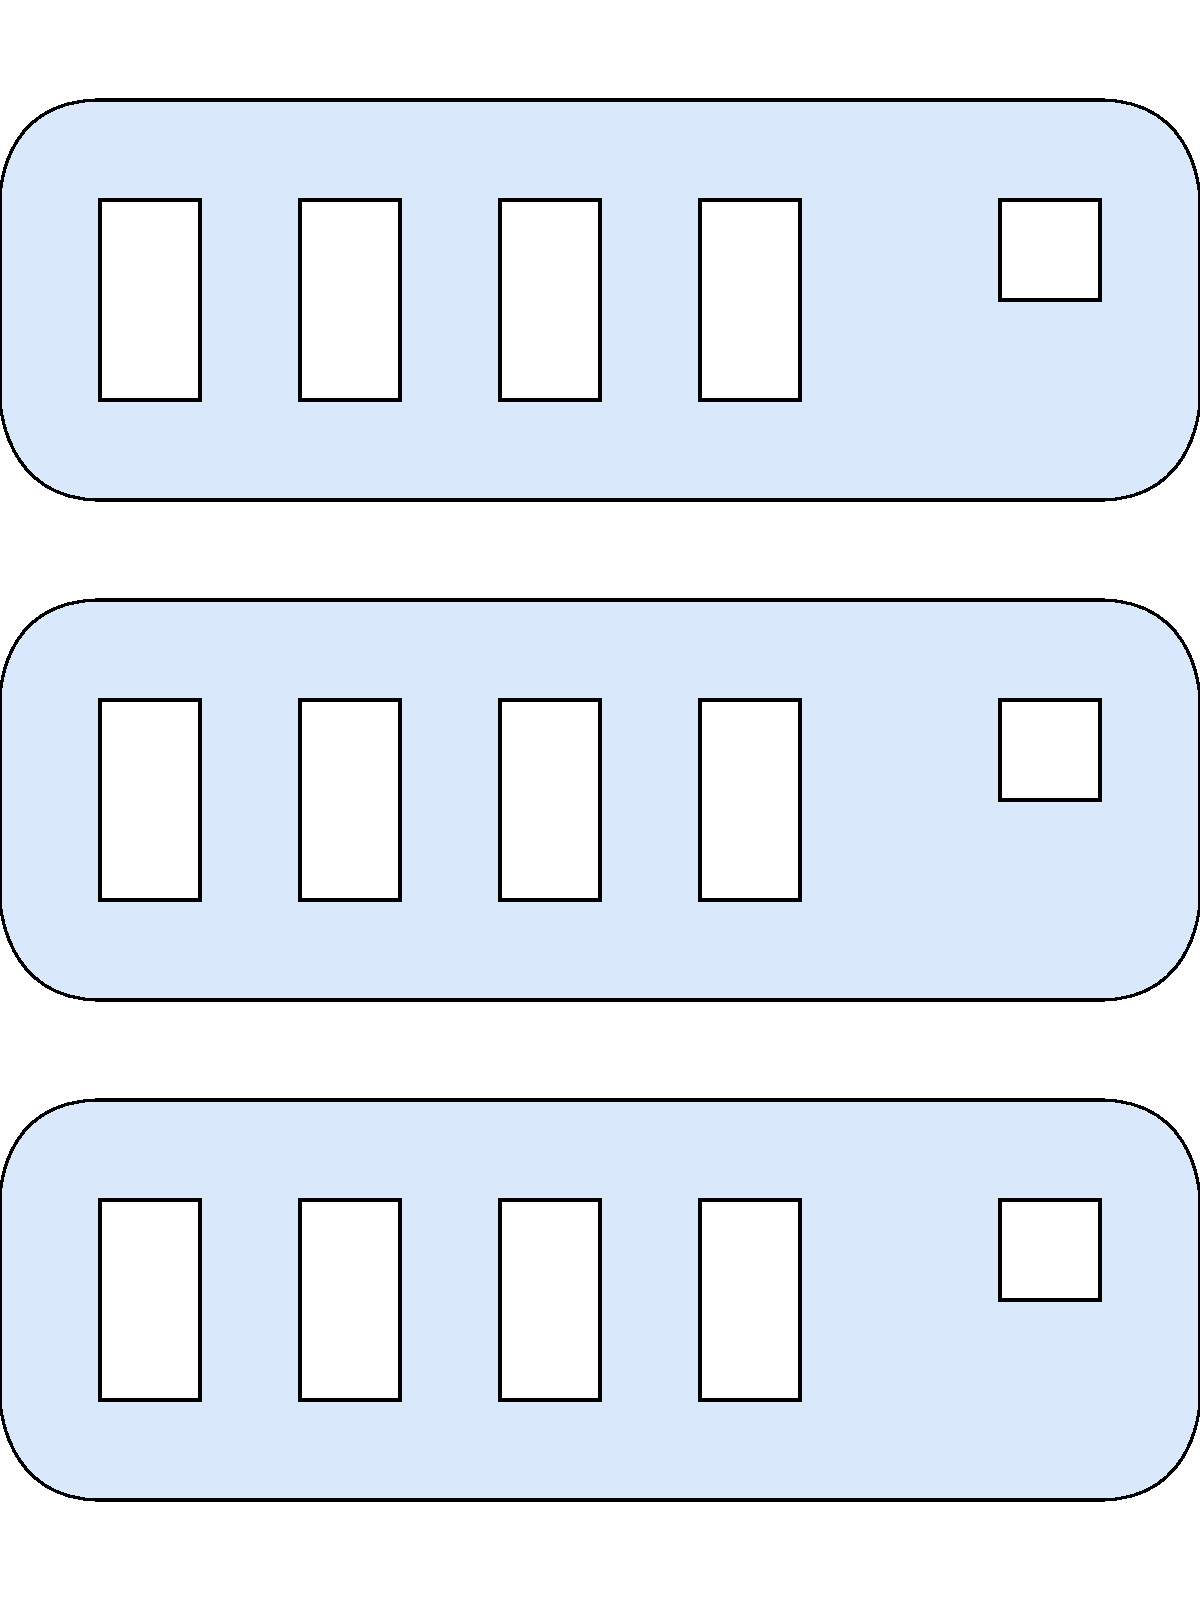
\includegraphics[scale=0.05]{img/blue-node.pdf}};
        \node[below=3pt of A] {\textbf{A}};
        \node<1>[above=3pt of A] {\includegraphics[scale=0.4]{img/doc.pdf}};
        \node<2-4>[above=3pt of A] {\includegraphics[scale=0.4]{img/docA.pdf}};
        \node<5->[above=3pt of A] {\includegraphics[scale=0.4]{img/docABC.pdf}};

        \node (B) at (-2, -3) {\includegraphics[scale=0.05]{img/red-node.pdf}};
        \node[below=3pt of B] {\textbf{B}};
        \node<1-2>[left=3pt of B] {\includegraphics[scale=0.4]{img/doc.pdf}};
        \node<3>[left=3pt of B] {\includegraphics[scale=0.4]{img/docA.pdf}};
        \node<4>[left=3pt of B] {\includegraphics[scale=0.4]{img/docAB.pdf}};
        \node<5->[left=3pt of B] {\includegraphics[scale=0.4]{img/docABC.pdf}};

        \transparent{0.2}\node<-4> (C) at (2, -3) {\includegraphics[scale=0.05]{img/green-node.pdf}};
        \transparent{1}\node<4-> at (2, -3) {\includegraphics[scale=0.05]{img/green-node.pdf}};
        \node[below=3pt of C] {\textbf{C}};
        \node<1-3>[right=3pt of C] {\includegraphics[scale=0.4]{img/transparent-doc.pdf}};
        \node<4>[right=3pt of C] {\includegraphics[scale=0.4]{img/docC.pdf}};
        \node<5->[right=3pt of C] {\includegraphics[scale=0.4]{img/docABC.pdf}};

        \draw[shorten >=3pt, shorten <=3pt]
          (A) to[bend right] (B)
          (B) to[bend right] (C)
          (C) to[bend right] (A);

        \node<2>[below left=-30pt and 5pt of A] {\includegraphics[scale=0.4]{img/updateA.pdf}};
        \node<2, 4>[below right=-30pt and 5pt of A] {\includegraphics[scale=0.4]{img/updateA.pdf}};

        \node<4>[below right=-4pt and 1pt of B] {\includegraphics[scale=0.4]{img/updateB.pdf}};
        \node<4>[above left=1pt and -15pt of B] {\includegraphics[scale=0.4]{img/updateB.pdf}};

        \node<4>[below left=-4pt and 1pt of C] {\includegraphics[scale=0.4]{img/updateC.pdf}};
        \node<4>[above right=1pt and -15pt of C] {\includegraphics[scale=0.4]{img/updateC.pdf}};
      \end{tikzpicture}
    \end{column}
    \begin{column}{0.35\textwidth}
      \begin{itemize}
        \item Replicated data structure
        \item<2-> Updates performed without coordination
        \item<5-> Eventual consistency
      \end{itemize}
    \end{column}
  \end{columns}
\end{frame}

\begin{frame}{Large-scale system}
  \begin{center}
    \begin{tikzpicture}
      \node (A) {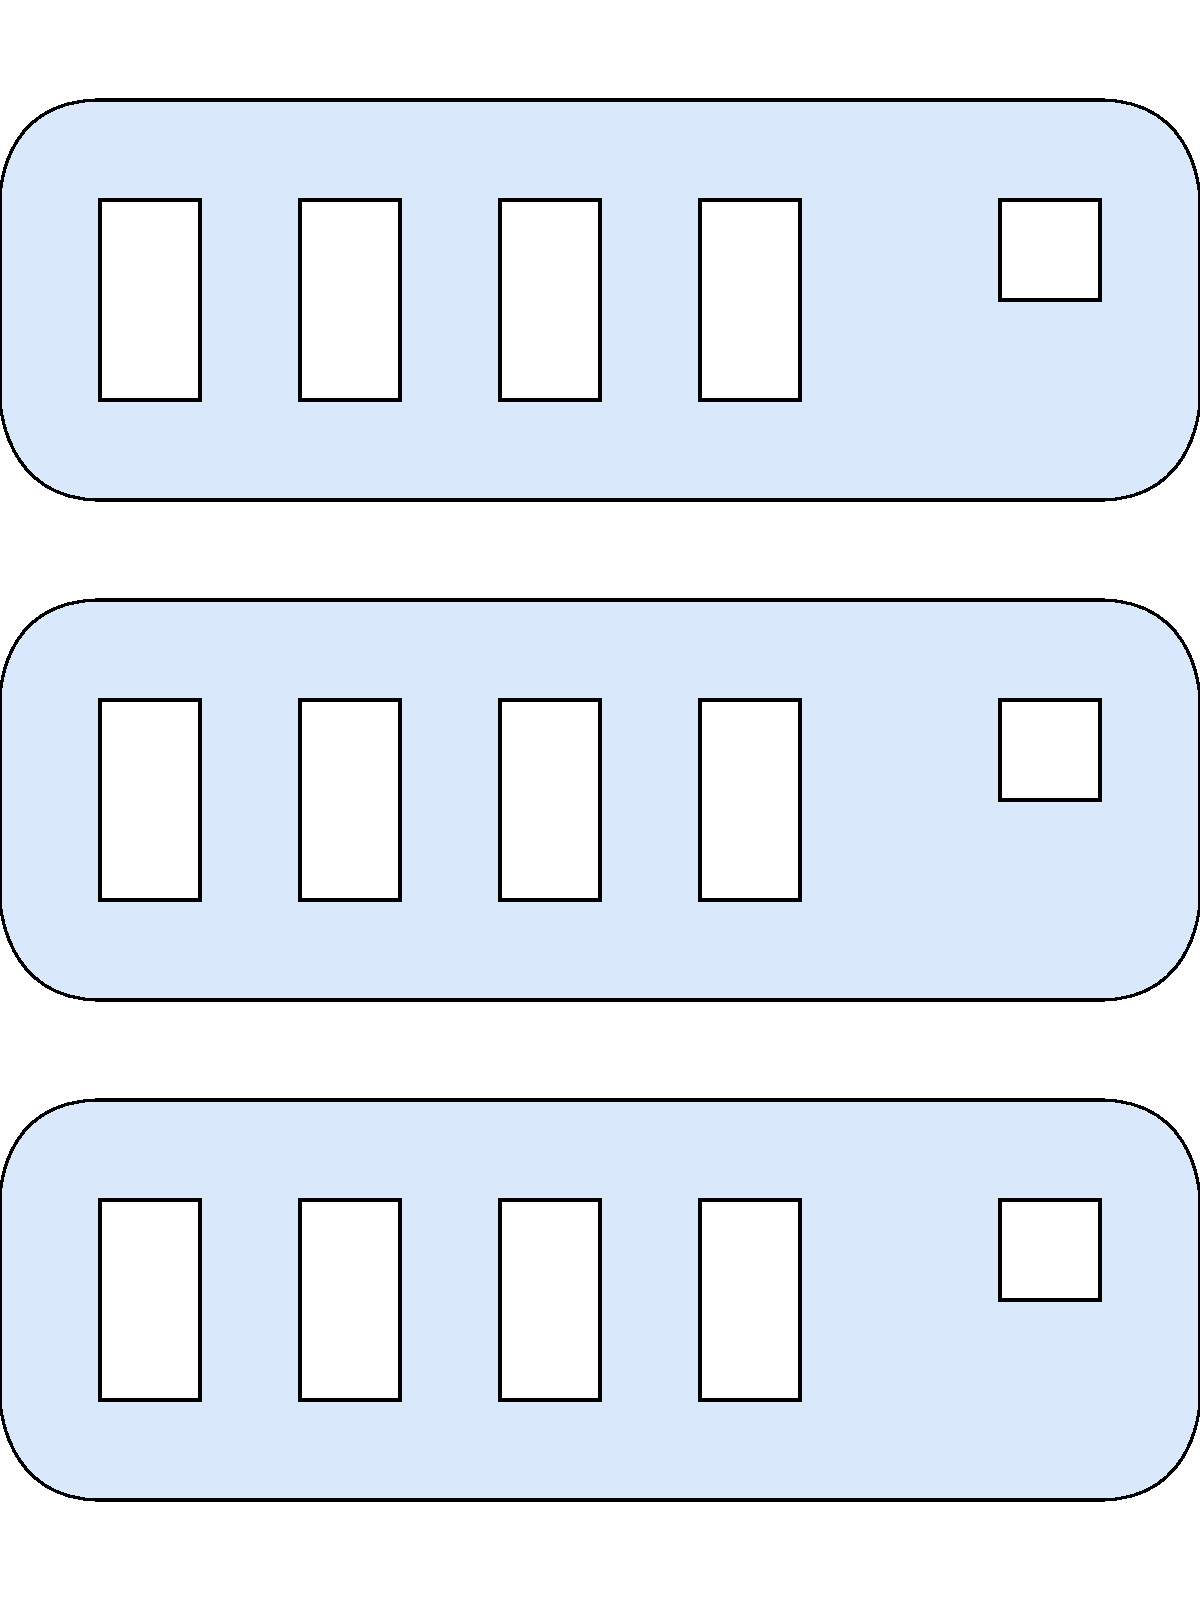
\includegraphics[scale=0.05]{img/blue-node.pdf}};
      \node[below left=0.5 and -0.2 of A] (B) {\includegraphics[scale=0.05]{img/red-node.pdf}};
      \node[below right=0.5 and -0.2 of A] (C) {\includegraphics[scale=0.05]{img/green-node.pdf}};

      \node[above left=0.5 and -0.2 of B] (D) {
\includegraphics[scale=0.05]{img/black-node.pdf}};
      \transparent{0.2}\node[below left=0.5 and -0.2 of D] (E) {
\includegraphics[scale=0.05]{img/black-node.pdf}};
      \transparent{1}\node[above left=0.5 and -0.2 of D] (H) {
\includegraphics[scale=0.05]{img/black-node.pdf}};
      \node[above right=0.5 and -0.2 of D] (I) {
\includegraphics[scale=0.05]{img/black-node.pdf}};

      \transparent{0.2}\node[above right=0.5 and -0.2 of C] (F) {
\includegraphics[scale=0.05]{img/black-node.pdf}};
      \transparent{1}\node[below right=0.5 and -0.2 of F] (G) {
\includegraphics[scale=0.05]{img/black-node.pdf}};
      \node[above right=0.5 and -0.2 of F] (J) {
\includegraphics[scale=0.05]{img/black-node.pdf}};
      \node[above left=0.5 and -0.2 of F] (K) {
\includegraphics[scale=0.05]{img/black-node.pdf}};

      \node[below left=0.5 and -0.2 of B] (M) {
\includegraphics[scale=0.05]{img/black-node.pdf}};
      \node[below right=0.5 and -0.2 of C] (N) {
\includegraphics[scale=0.05]{img/black-node.pdf}};

      \node[left=of E] (O) {};
      \node[left=of H] (P) {};

      \node[right=of G] (Q) {};
      \node[right=of J] (R) {};

      \draw
      (A) -- (B)
      (B) -- (C)
      (C) -- (A)

      (B) -- (D)
      (D) -- (E)
      (E) -- (M)
      (B) -- (M)

      (A) -- (I)
      (I) -- (D)
      (D) -- (H)

      (C) -- (F)
      (F) -- (G)
      (G) -- (N)
      (N) -- (C)

      (A) -- (K)
      (K) -- (F)
      (F) -- (J)

      (E) -- (O)
      (H) -- (P)
      (G) -- (Q)
      (J) -- (R);
    \end{tikzpicture}
  \end{center}
\end{frame}

\begin{frame}{Identifier-based \acp{CRDT}}
  \begin{block}{Identifiers}
    \begin{itemize}
      \item Attached to elements and updates
      \item Have to comply to several constraints
      \begin{itemize}
        \item Unique
        \item Immutable
        \item Order relation
        \item Many others
      \end{itemize}
      \item Achieve transaction-less and commutative updates
    \end{itemize}
  \end{block}
  \begin{alertblock}{Limits}<2->
    \begin{itemize}
      \item Unbounded size of identifiers
      % TODO: Soit ils grossissent très vite, soit tombstones
      \item Efficiency decreasing over time
    \end{itemize}
  \end{alertblock}
\end{frame}

\begin{frame}{Research problem}
  \begin{block}{Reduce size of identifiers}
    \begin{itemize}
      \item Renaming problem\cite{AlistarhAGG2011}
    \end{itemize}
  \end{block}
  \begin{alertblock}<2->{Make identifiers mutable again}
    \begin{itemize}
      \item Trade-off mutability/immutability
    \end{itemize}
  \end{alertblock}
\end{frame}

\begin{frame}[standout]
  Thanks for your attention, any questions?
  \vspace{3em}
  \begin{center}
    \ccby
  \end{center}
\end{frame}

% TODO: Faire une slide de back-up

\begin{frame}[allowframebreaks]{References}
	\bibliography{biblio}
	\bibliographystyle{abbrv}
\end{frame}

\end{document}
